\documentclass[11pt]{article}

\usepackage[a4paper, margin=1in]{geometry}
\usepackage{graphicx}
\usepackage{booktabs}
\usepackage{float}
\usepackage{setspace}
\usepackage{lineno}
\usepackage{caption}
\usepackage{natbib}
\usepackage{amsmath}
\usepackage{subcaption}

\onehalfspacing
\linenumbers

% Word count settings
%TC:envir titlepage 0 0
%TC:envir thebibliography 0 0
\newcommand{\wordcount}{\input{wordcount.txt}}

\title{Logistic growth models best describe most microbial growth curves, whereas cubic models capture post-peak decline}
\author{Yian Liu}
\date{March 2026}

\bibliographystyle{apalike}

\begin{document}

\begin{titlepage}
    \nolinenumbers
    \centering
    \vspace*{\fill}

    {\LARGE Logistic growth models best describe most microbial growth\\
    curves, whereas cubic models capture post-peak decline\par}

    \vspace{1.5cm}

    {\Large Yian Liu\par}

    \vspace{0.3cm}

    {\large Imperial College London\par}

    \vspace{0.8cm}

    {\large March 2026\par}

    \vspace{1.2cm}

    {\large Word count: \wordcount \par}

    \vspace*{\fill}
\end{titlepage}

\linenumbers

\begin{abstract}
Microbial growth curves are often nonlinear and can differ substantially in shape across datasets. This variation creates the need to compare models that differ not only in flexibility but also in biological interpretability. Here we ask which of the three candidate models best describes microbial growth curves in a heterogeneous dataset: the logistic growth model, the quadratic polynomial, or the cubic polynomial. We analysed 305 cleaned growth curves spanning four measurement units and fitted each candidate model to each curve. Model support was evaluated using the Akaike Information Criterion (AIC) and the Bayesian Information Criterion (BIC), with convergence summarised separately. The logistic growth model was selected most often under both AIC and BIC, whereas the cubic model was the main alternative and the quadratic model won only a small minority of curves. Representative fitted curves showed that logistic performed best for clear sigmoidal trajectories, while cubic became more competitive when post-peak decline was present. Overall, the logistic growth model provided the best general description of microbial growth in this dataset, but the cubic model remained important when empirical curves departed from a simple sigmoidal form.
\end{abstract}

\section{Introduction}
Microbial population growth is a fundamental biological process because changes in population density affect resource use, competition, and spoilage-related dynamics. In batch culture, microbial populations typically pass through a series of phases, including an initial lag phase, a period of rapid exponential growth, and a stationary phase as resources become scarce \citep{Monod1949,Zwietering1990}. These phase transitions mean that growth trajectories usually change nonlinearly over time. Therefore, models that describe the full population growth curve are more informative than approaches that estimate growth patterns from a visually selected exponential segment.

Accordingly, a core question is not only whether a model can fit a curve, but also whether it can provide an effective description of the biological pattern observed in the data. The parameters of  mechanistic growth models such as the logistic growth model usually have clear biological meanings. Some parameters describe how fast a population grows, whereas others describe the maximum population size that can be reached under resource limitation. By contrast, polynomial models can flexibly summarize curved trajectories without requiring the fitted parameters to map directly onto specific biological processes \citep{WhiteMarshall2019}.

This distinction is useful because empirical microbial growth curves often differ in shape. Some curves show a clear sigmoidal trajectory, whereas others are less strongly curved or even decline after reaching a peak. Therefore, even if a model makes more biological sense, it is not always the best at capturing every real growth curve.

Here we compare one mechanistic nonlinear model, the logistic growth model, with two phenomenological models, quadratic and cubic models, to evaluate which model best describes microbial growth curves in a heterogeneous dataset. We compare candidate models using the Akaike Information Criterion (AIC) and the Bayesian Information Criterion (BIC), rather than treating model comparison as a simple significance-testing exercise. These criteria provide an information-theoretic framework for assessing the relative support for competing biological models \citep{JohnsonOmland2004}. Specifically, we explore whether the logistic growth odel provides the best description of microbial growth overall, and whether more flexible polynomial models become more advantageous when curve shape departs from a simple sigmoidal form, especially when post-peak decline is present.

\section{Methods}

\subsection{Data and preprocessing}

We used \texttt{logistic\_growth\_data.csv} as the starting dataset. The response variable was \texttt{PopBio}, which records population or biomass measurements, and the predictor variable was \texttt{Time}. Additional metadata included temperature, measurement units, species, growth medium, replicate identity, and source citation. Following the project specification, we treated each unique combination of \texttt{Species}, \texttt{Temp}, \texttt{Medium}, \texttt{Citation}, and \texttt{Rep} as one microbial growth curve. We concatenated these fields to form a character identifier (\texttt{curve\_id}) and then assigned each curve a numeric index (\texttt{curve\_num}). Before fitting, we parsed numeric values from the \texttt{Time}, \texttt{PopBio}, and \texttt{Temp} columns and removed records with non-finite \texttt{Time} or \texttt{PopBio}. When repeated measurements occurred at the same time point within the same curve, we averaged \texttt{PopBio} across those records so that each curve had at most one observation per time value.

For model fitting, time was centred within each curve as

\begin{equation}
t = \mathrm{Time} - \min(\mathrm{Time}),
\label{eq:tcenter}
\end{equation}

so that all candidate models were fitted on a comparable within-curve time scale starting at zero. We also generated exploratory summaries before model fitting. These included a unit-level count table, a curve-level flag table, a random sample of 20 point-only growth curves, a full spaghetti plot of all curves, and a log-scale version of the same 20 sampled curves for observations with positive \texttt{PopBio}. These exploratory outputs were used to understand variation in curve shape and to identify features such as non-positive values and approximate post-peak decline.

\subsection{Candidate models}

We compared three candidate models. The first two were phenomenological polynomial models: a quadratic polynomial,

\begin{equation}
y_t = b_0 + b_1 t + b_2 t^2,
\label{eq:quadratic}
\end{equation}

and a cubic polynomial,

\begin{equation}
y_t = b_0 + b_1 t + b_2 t^2 + b_3 t^3.
\label{eq:cubic}
\end{equation}

These models are flexible and can capture curved trajectories, including post-peak decline, but their coefficients do not map directly onto specific biological processes.

The third model was a mechanistic nonlinear model, the logistic growth model,

\begin{equation}
y_t = \frac{K}{1 + \left(\frac{K - N_0}{N_0}\right)e^{-rt}},
\label{eq:logistic}
\end{equation}

where $N_0$ is the initial abundance, $r$ is the growth-rate parameter, and $K$ is the upper asymptote or carrying-capacity parameter. Although the code file also contains an optional Gompertz fitting branch, this was disabled in the present analysis (\texttt{DO\_GOMPERTZ = FALSE}), so only the three models in Eqs.~\ref{eq:quadratic}--\ref{eq:logistic} were compared.

\subsection{Model fitting and selection}

The quadratic and cubic models were fitted using ordinary least squares with \texttt{lm()}. Specifically, Eq.~\ref{eq:quadratic} was fitted as \texttt{PopBio \textasciitilde{} t + I(t\textasciicircum 2)} and Eq.~\ref{eq:cubic} as \texttt{PopBio \textasciitilde{} t + I(t\textasciicircum 2) + I(t\textasciicircum 3)}. The logistic growth model in Eq.~\ref{eq:logistic} was fitted with \texttt{nlsLM()} from the \texttt{minpack.lm} package, which implements a Levenberg--Marquardt nonlinear least-squares procedure and supports parameter bounds \citep{Elzhov2023,More1978}. This choice was appropriate because nonlinear least-squares fitting requires explicit starting values and can be sensitive to poor initialization or overly restrictive parameter ranges \citep{Baty2015}.

Starting values for the logistic growth model were chosen separately for each curve using simple data-driven rules. The initial abundance parameter $N_0$ was initialized from the smallest positive observed \texttt{PopBio} value, with a small positive fallback when necessary. The carrying-capacity parameter $K$ was initialized from the observed maximum \texttt{PopBio} value and adjusted upward if that value was not greater than the starting value of $N_0$. The growth-rate parameter $r$ was initialized from the maximum slope of successive differences in $\log(\texttt{PopBio})$ over centred time for positive observations, when enough positive data were available; otherwise a default positive value was used. Lower bounds were set to keep $N_0$ and $K$ positive and $r$ non-negative, while upper bounds were set as broad multiples of the curve-specific starting values. We allowed up to 200 iterations for each nonlinear fit.

To reduce fitting failures, we screened the curves for minimum data requirements before fitting. Quadratic fits were not attempted when the number of unique time points was less than or equal to the number of model parameters ($k=3$), and cubic fits were not attempted when the number of unique time points was less than or equal to four. Logistic fits were not attempted when there were too few unique time points or fewer than six total observations. All fitting routines were wrapped in \texttt{tryCatch()}, so failed fits were retained in the output and recorded as non-converged rather than silently dropped.

For every fitted model, we exported parameter estimates and several fit summaries. The primary model selection criteria were the Akaike Information Criterion (AIC) and the Bayesian Information Criterion (BIC),

\begin{equation}
\mathrm{AIC} = 2k - 2\log(\hat{L}),
\label{eq:aic}
\end{equation}

\begin{equation}
\mathrm{BIC} = k \log(n) - 2\log(\hat{L}),
\label{eq:bic}
\end{equation}

where $k$ is the number of fitted parameters, $n$ is the number of observations, and $\hat{L}$ is the maximized likelihood \citep{JohnsonOmland2004}. For each curve, we identified the best-supported model separately under AIC and BIC by selecting the converged fit with the smallest value of the corresponding information criterion. We also saved the residual sum of squares,

\begin{equation}
\mathrm{RSS} = \sum_{i=1}^{n}(y_i - \hat{y}_i)^2,
\label{eq:rss}
\end{equation}

and the coefficient of determination,

\begin{equation}
R^2 = 1 - \frac{\mathrm{RSS}}{\sum_{i=1}^{n}(y_i - \bar{y})^2},
\label{eq:r2}
\end{equation}

as auxiliary summaries. However, RSS and $R^2$ were not used as the primary basis for model choice. After fitting, we summarised convergence rates by model, counted the number of AIC and BIC wins for each model, generated predicted values across a 200-point grid within each observed time range, and overlaid the fitted lines on each empirical curve. Finally, we selected four representative fitted curves for the main text by combining AIC winner identity, the AIC difference between the best and second-best model, and exploratory flags for decline and non-positive values.

\subsection{Computing tools}

R was the main analytical language used in this study because it provides a convenient and reproducible environment for data wrangling, exploratory plotting, linear modelling, nonlinear least-squares fitting, and result summarisation. In particular, \texttt{readr}, \texttt{dplyr}, \texttt{tidyr}, \texttt{purrr}, and \texttt{stringr} were used for data import and preprocessing; \texttt{ggplot2} was used for exploratory and fitted-curve visualisation; \texttt{here} was used to manage project-relative file paths; and \texttt{minpack.lm} was used to fit the logistic growth model with the \texttt{nlsLM()} function because it provides a more robust nonlinear least-squares algorithm than base \texttt{nls()} and allows parameter bounds.

Bash was used to support reproducibility by running the full workflow from a single entry point (\texttt{run\_MiniProject.sh}), including data preparation, model fitting, analysis, figure selection, and report compilation where available. The manuscript was written in \LaTeX{} because it provides precise control over scientific formatting, equations, citations, and figure placement. References were managed with Bib\TeX{}, which allowed the bibliography and in-text citations to be handled consistently and reproducibly.

\section{Results}

\subsection{Overview of dataset heterogeneity}

The cleaned dataset comprised 305 microbial growth curves measured in four population units: CFU, DryWeight, N and OD\_595 (Figure 1). Visual inspection of all curves showed substantial heterogeneity in both numerical scale and trajectory shape. Curves measured as N and CFU often extended to much larger values than those measured as OD\_595 or DryWeight, and the observed time ranges also varied considerably among datasets. As a result, the dataset did not consist of one uniform type of growth trajectory.

This heterogeneity was visible not only in the vertical scale of the data, but also in the overall form of the curves. Some curves showed a clear sigmoidal pattern, with an initial rise followed by an apparent plateau. Others were more weakly curved, appeared closer to a simple hump-shaped trajectory, or showed an obvious decline after reaching a maximum value. In some cases, the increase was steep and concentrated over a narrow time window, whereas in other cases the change in population density was more gradual across a longer interval. These differences indicated that the empirical data included both curves that were broadly consistent with the shape expected under a logistic growth process and curves that departed from this form.

The overview of all fitted trajectories therefore provided an important context for model comparison. Because the dataset contained substantial variation in scale, shape, it was unlikely that a single candidate model would describe every curve equally well. This made it necessary to compare the logistic growth model against the two polynomial alternatives across the full set of curves.
\begin{figure}[H]
\centering
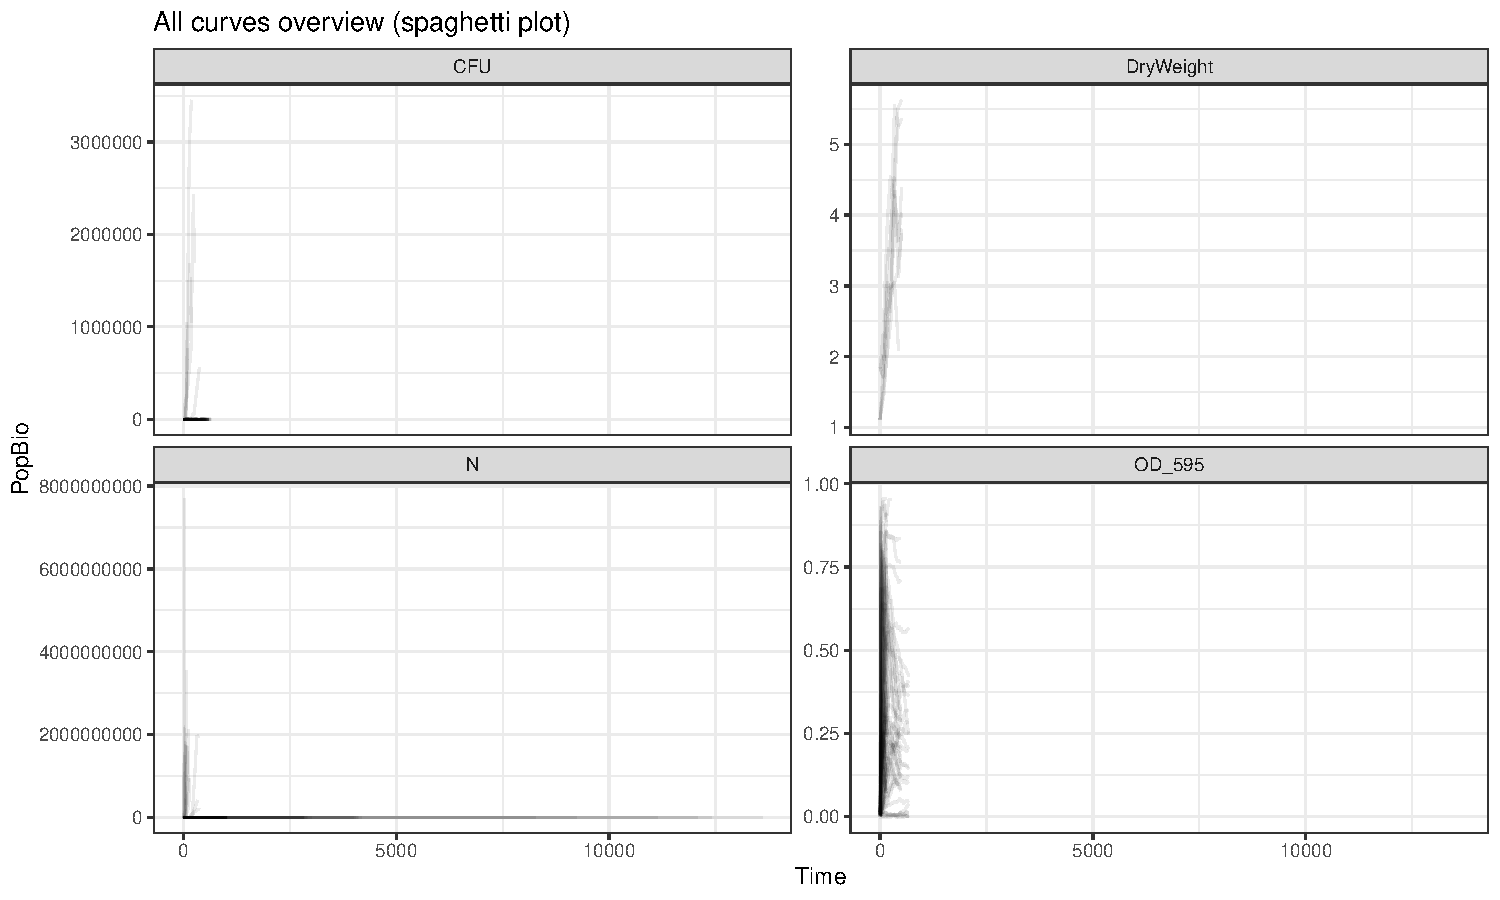
\includegraphics[width=0.9\textwidth]{plots/eda_all_spaghetti.pdf}
\caption{Overview of all cleaned growth curves, faceted by measurement unit. The figure shows strong heterogeneity in both scale and shape across CFU, DryWeight, N, and OD 595 curves.}
\label{fig:spaghetti}
\end{figure}

\subsection{Overall model comparison}

Overall model-selection results showed a clear and consistent ranking of the three candidate models (Table 1). Across all 305 curves, the logistic growth model was selected most often under both information criteria. Under AIC, logistic growth model was the best-supported model for 185 curves (60.7\%), compared with 85 curves (27.9\%) for the cubic model and 35 curves (11.5\%) for the quadratic model. The same overall ordering was obtained under BIC, where logistic growth model won 188 curves (61.6\%), cubic model won 80 curves (26.2\%), and quadratic model won 37 curves (12.1\%).

These results indicate that the overall pattern was stable across both model-selection criteria. Regardless of whether AIC or BIC was used, the logistic growth model was selected most frequently, the cubic model was the main alternative, and the quadratic model was selected least often. The difference between AIC and BIC affected only a small number of curves and did not change the overall hierarchy of model support.

\begin{table}[H]
\centering
\caption{Overall model performance across all growth curves. Logistic growth model was the most frequently selected model under both AIC and BIC, whereas quadratic and cubic models showed higher convergence rates.}
\label{tab:model_summary}
\begin{tabular}{lccc}
\toprule
Model & AIC wins & BIC wins & Convergence \\
\midrule
Logistic  & 185 (60.7\%) & 188 (61.6\%) & 285/305 (93.4\%) \\
Cubic     & 85 (27.9\%)  & 80 (26.2\%)  & 299/305 (98.0\%) \\
Quadratic & 35 (11.5\%)  & 37 (12.1\%)  & 305/305 (100.0\%) \\
\bottomrule
\end{tabular}
\end{table}

The convergence summary revealed a different pattern from the model-selection summary (Figure 2). Quadratic fits converged for all 305 curves (100.0\%), cubic fits converged for 299 curves (98.0\%), and logistic fits converged for 285 curves (93.4\%). Thus, the polynomial models were numerically more stable than the logistic growth model, even though they were selected less often overall.

\begin{figure}[H]
\centering
\begin{subfigure}[b]{0.48\textwidth}
    \centering
    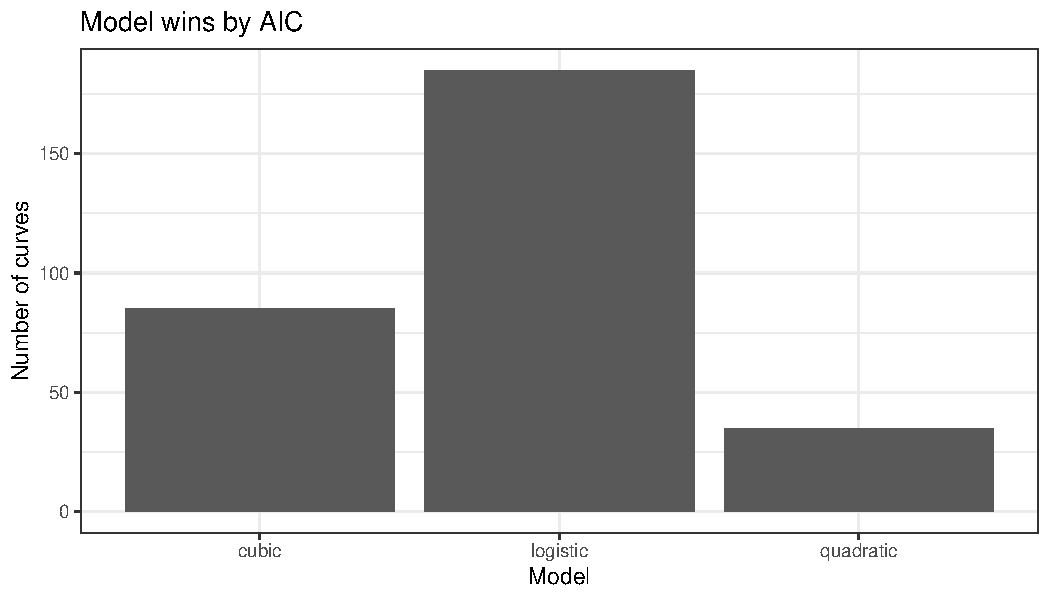
\includegraphics[width=\textwidth]{plots/model_wins_AIC.pdf}
    \caption{Model wins by AIC}
    \label{fig:wins_aic}
\end{subfigure}
\hfill
\begin{subfigure}[b]{0.48\textwidth}
    \centering
    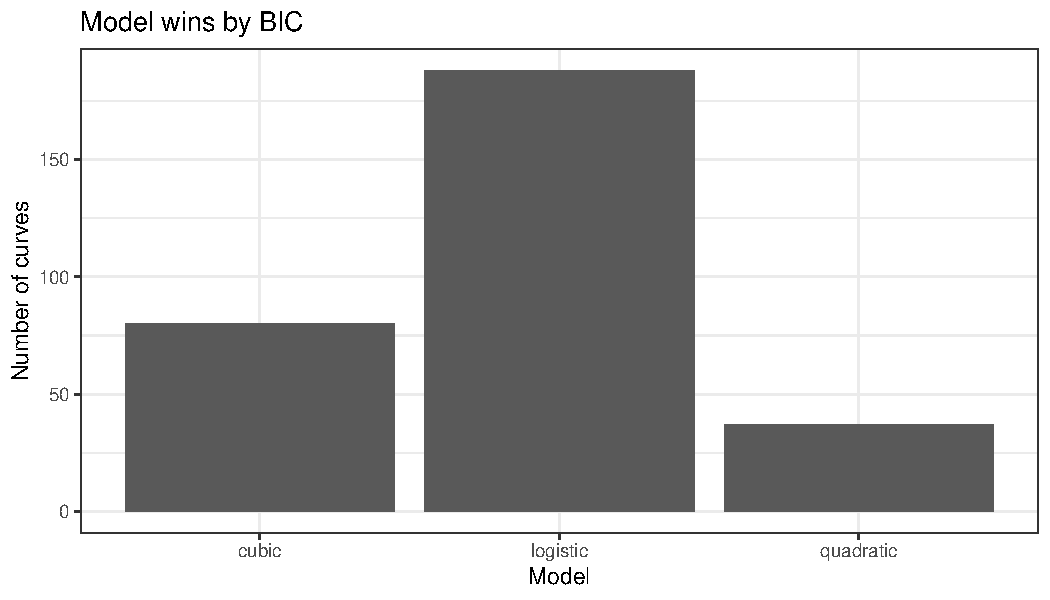
\includegraphics[width=\textwidth]{plots/model_wins_BIC.pdf}
    \caption{Model wins by BIC}
    \label{fig:wins_bic}
\end{subfigure}
\caption{Overall model selection outcomes under two information criteria. In both panels, the logistic growth model was selected most often, followed by the cubic model and then the quadratic model.}
\label{fig:model_wins}
\end{figure}

Taken together, these results show a clear dataset-level hierarchy. The logistic growth model provided the best overall description for most curves, the cubic model accounted for a substantial minority of best-supported fits, and the quadratic model contributed only a small proportion of wins. At the same time, the convergence results show that fitting stability and model support were not identical outcomes. This made it useful to examine representative fitted curves in more detail.

\subsection{Representative fitted curves}

The four representative fitted curves show the main patterns behind the overall results (Figure 3). The first case (Figure 3a) shows a clear example in which the logistic growth model performed best. In this curve, the observed points follow a typical sigmoidal pattern. The values rise quickly at first and then level off at an upper plateau. The logistic fit follows this pattern closely. By contrast, the polynomial models give less convincing fits. This example shows a common situation in which the mechanistic nonlinear model was strongly supported.

The second case (Figure 3b) shows the opposite pattern. In this example, the cubic model performed best. The trajectory rises and then declines after reaching a higher value. This shape does not match a simple monotonic approach to an asymptote. The cubic model captures both the increase and the later decline more closely than the logistic growth model. This example shows the main situation in which the cubic model became the strongest alternative to the logistic growth model.

The other two panels (Figure 3c and Figure 3d) show borderline cases. In these cases, the best model was only slightly better supported than the others. In the borderline logistic case, the logistic growth model was selected as the best model. However, the logistic and cubic curves remain visually similar across much of the observed range. This result suggests that some model wins were not linked to large differences in curve shape. In the borderline quadratic case, the quadratic model was selected. However, the three fitted curves are still fairly similar overall. The winning model is not separated from the others as clearly as in the stronger examples.

These representative curves add detail to the overall summaries by showing how the results looked for individual trajectories. They show that the strong overall performance of the logistic growth model mainly came from curves with a clear sigmoidal shape. They also show that the cubic model became more competitive when the trajectory included decline after the peak. At the same time, these examples show that not every best-model result was equally strong. Some curves had a clear winner, but others showed only small differences between competing models.
\begin{figure}[H]
\centering
\begin{subfigure}[b]{0.48\textwidth}
    \centering
    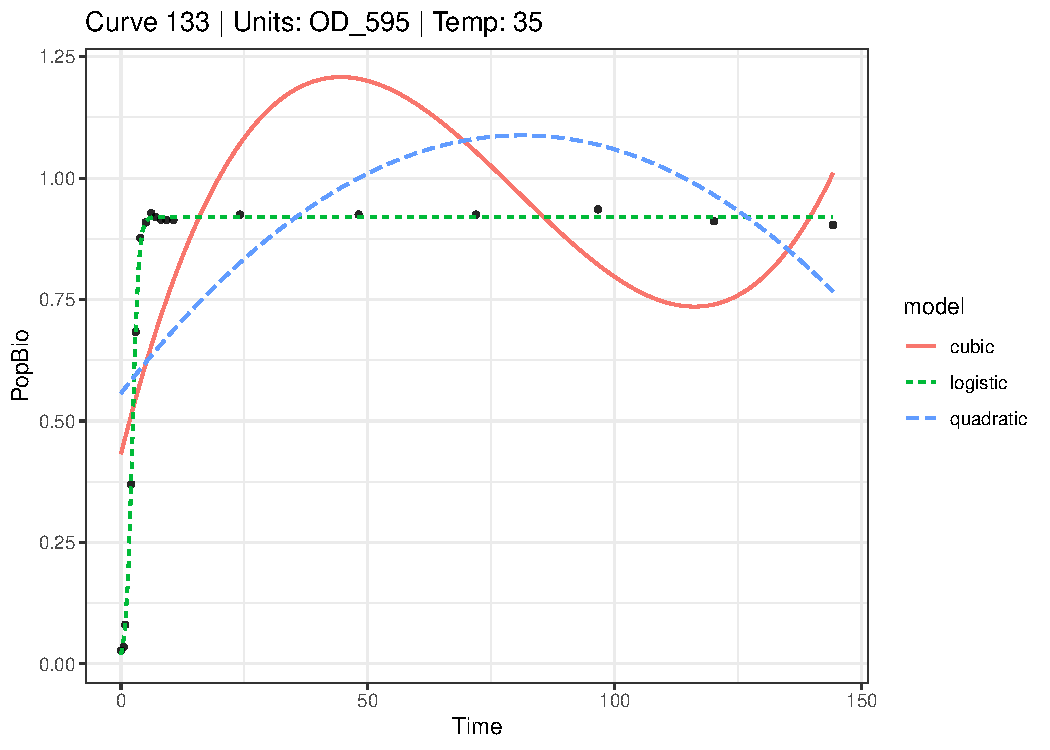
\includegraphics[width=\textwidth]{plots/curve_133.pdf}
    \caption{Curve 133: strong logistic win}
    \label{fig:curve133}
\end{subfigure}
\hfill
\begin{subfigure}[b]{0.48\textwidth}
    \centering
    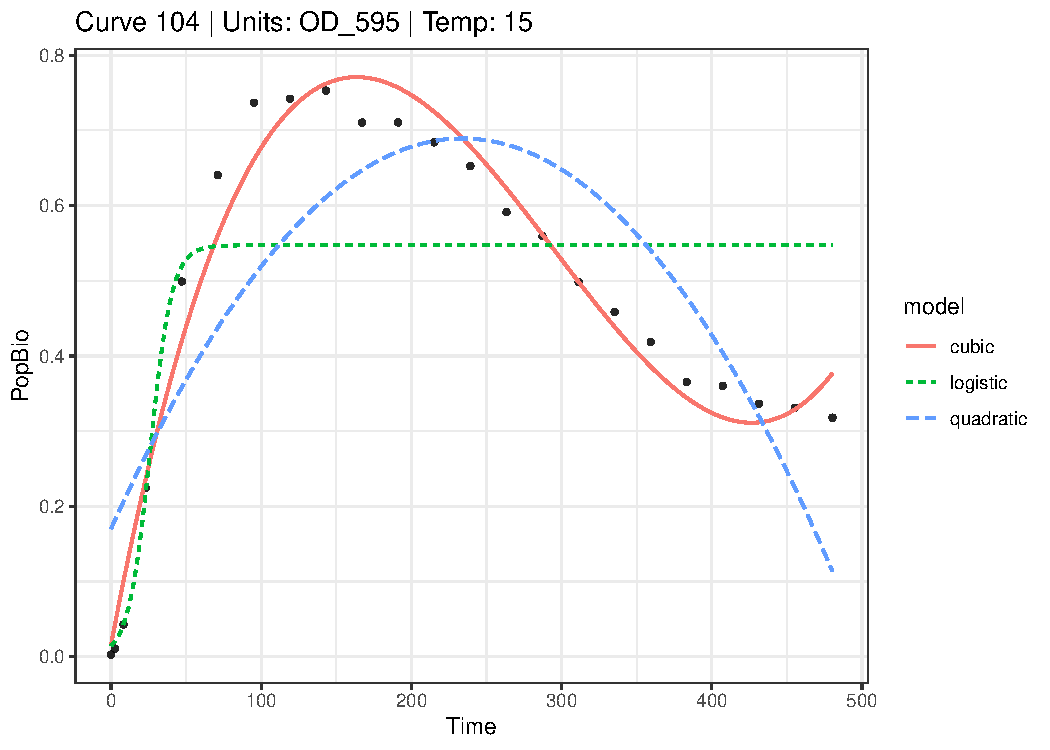
\includegraphics[width=\textwidth]{plots/curve_104.pdf}
    \caption{Curve 104: strong cubic win}
    \label{fig:curve104}
\end{subfigure}

\vspace{0.6em}

\begin{subfigure}[b]{0.48\textwidth}
    \centering
    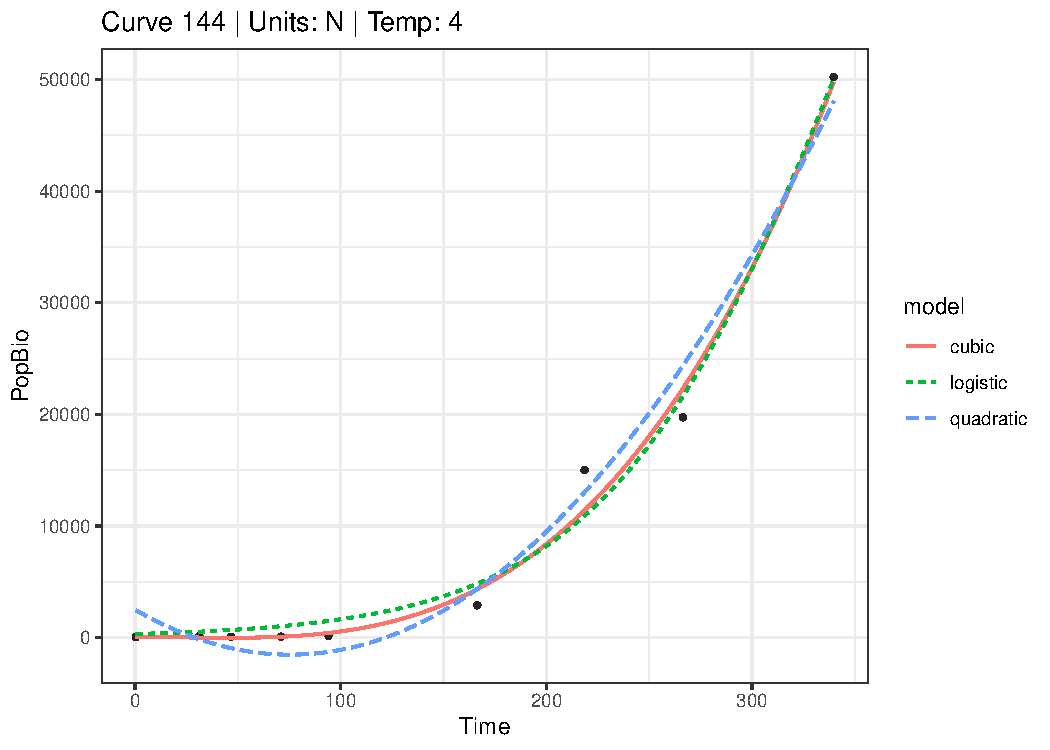
\includegraphics[width=\textwidth]{plots/curve_144.pdf}
    \caption{Curve 144: borderline logistic case}
    \label{fig:curve144}
\end{subfigure}
\hfill
\begin{subfigure}[b]{0.48\textwidth}
    \centering
    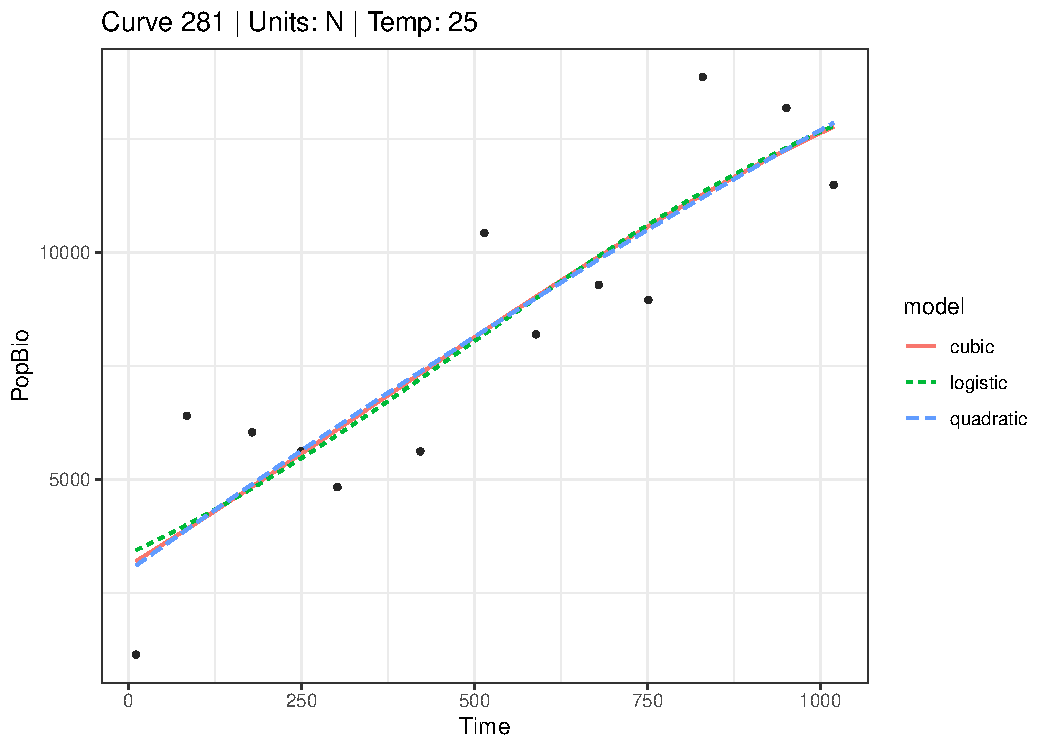
\includegraphics[width=\textwidth]{plots/curve_281.pdf}
    \caption{Curve 281: borderline quadratic case}
    \label{fig:curve281}
\end{subfigure}
\caption{Representative fitted curves selected to illustrate the main outcome patterns. Black points show the observed data for each microbial growth curve, and coloured lines show fitted values from the three candidate models. Panel (a) shows a clean sigmoidal trajectory strongly favoured by the logistic growth model. Panel (b) shows a curve with clear post-peak decline that was better captured by the cubic model. Panels (c) and (d) show borderline cases in which the best-supported model was only weakly separated from the alternatives.}
\label{fig:rep_curves}
\end{figure}

\section{Discussion}

The results showed a clear overall pattern. The logistic growth model was selected most often under both AIC and BIC. The cubic model was the main alternative. The quadratic model won only a small minority of curves. This pattern matters because model comparison is not only a technical exercise. Different models represent different biological ideas, and information criteria allow those alternatives to be compared directly rather than through a single null-hypothesis test \citep{JohnsonOmland2004}.

The logistic growth model probably won most often because many curves in the dataset still followed the basic logic of density-dependent growth. In batch culture, microbial populations usually increase rapidly when resources are still available and then slow as resources become limiting. The logistic growth model captures that sigmoidal pattern directly. Logistic growth model also has parameters with clear biological meanings. This feature is one reason mechanistic models are often attractive in ecology and evolution \citep{Zwietering1990,WhiteMarshall2019}. In the dataset, many curves showed a clear rise and an apparent plateau. That shape matches the structure of the logistic growth model. So the overall success of logistic is biologically sensible, not just statistically convenient.

The cubic model became more competitive when curves showed post-peak decline. This result also makes biological sense. Batch cultures do not always stop at a stable plateau. Some populations move from stationary phase into a decline or death phase as nutrients are exhausted and cells die or recycle \citep{NavarroLlorens2010}. A logistic growth model does not represent that downward phase well, because it mainly describes a monotonic approach to an upper asymptote. The cubic model is different. It is more flexible within the observed data range, so it can bend upward and then downward. That flexibility helps it track decline-phase curves more closely. The cubic model can describe shape well, but the parameters do not provide the same direct biological interpretation as the logistic growth model \citep{WhiteMarshall2019}. This trade-off fits the representative curves in the Results section, where the strongest cubic example (Figure 3b) was also the clearest post-peak decline case.

The quadratic model mainly acted as a simple baseline. It converged very reliably, but it won relatively rarely. This pattern suggests that the quadratic model was often too simple to capture the full shape of a microbial growth curve. It could still perform reasonably in short series, in weakly curved trajectories, or in borderline cases where the competing models were only slightly different. However, it lacked the flexibility of the cubic model and the biological structure of the logistic growth model. For that reason, the quadratic model was useful as a comparison, but it was rarely the best biological description of the data.

This study also has clear limits. First, the dataset combines OD\_595, N, CFU, and DryWeight measurements across many species, media, and temperatures. That breadth is useful when the aim is to ask which model class suits which curve shape. It is less suitable when the aim is to compare fitted parameter values directly across all curves. Second, the nonlinear comparison was intentionally restricted to a single mechanistic nonlinear model, the logistic growth model. Other nonlinear alternatives, such as the Gompertz model, were not included in the final comparison. Therefore, the present conclusions apply to the specific candidate set examined here, rather than to all possible nonlinear growth models. Third, some best-model assignments were borderline. In those cases, a winning model was only weakly separated from its alternatives. Fourth, the lower convergence rate of the logistic growth model shows that numerical fit and biological relevance are not the same thing. Future work should extend the candidate set to models that represent lag and decline more explicitly, including additional nonlinear models where appropriate. Future work should also test whether the same overall ranking holds within subsets of curves defined by measurement unit or biological context. 

\clearpage
\bibliography{references}

\end{document}